\section{The Duffing oscillator}

\subsection{Analytical Ansatz}
As we have seen, Josephson junctions act as nonlinear inductors, hence adding nonlinearity, or anharmonicity, to an electrical circuit.
When the circuit is driven with low enough input power, the nonlinearity can be neglected.
In this case, the circuit can be described well by a driven harmonic oscillator,
\begin{align}
\ddot{x} + \delta \dot{x} + \alpha x = \gamma \cos(\omega t),
\end{align}
with the time-dependent displacement  $x=x(t)$, stiffness $\alpha$, damping $\delta$, drive amplitude $\gamma$ and drive frequency $\omega$.
All variables are assumed to be positive and real.
However, for most cases it is important to account for the anharmonicity.
The generalized mathematical model which describes such a circuit is the Duffing equation with the following equation of motion (EOM)\cite{hamelGeorgDuffingIngenieur1921}:
\begin{align}
\ddot{x} + \delta \dot{x} + \alpha x + \beta x^3 = \gamma \cos(\omega t),
\end{align}
with the anharmonicity $\beta$.

In fact, there exists an algebraic equation describing the amplitude response\cite{jordanNonlinearOrdinaryDifferential2007}:
\begin{align}
\left[ \left( \omega^2-\alpha-\frac{3}{4}\beta x^2 \right)^2 + \left( \delta\omega \right)^2 \right] x^2 = \gamma^2
\label{eq:Duffing-analytical}
\end{align}
We plot the solutions to a set of parameters ($\alpha=\gamma=1,\delta=0.1$) in Fig.\ref{fig:duffing}.

\begin{figure}
	\centering
	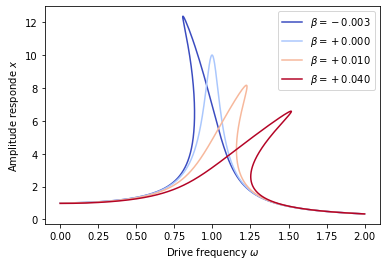
\includegraphics[width=0.7\linewidth]{chapter-theory/figs-general/duffing}
	\caption{Frequency response of Duffing oscillators for various nonlinearities and $\alpha=\gamma=1,\delta=0.1$, calculated from Eq.\ref{eq:Duffing-analytical}}
	\label{fig:duffing}
\end{figure}

\subsection{Intuitive Ansatz}
We can also take a more intuitive Ansatz to the above problem from which we can already gain qualitative information.
Let us assume the Duffing equation describes a mass on a (nonlinear) spring driven by a periodic external force.
Compared to the linear case with $F_r=kx$, the new restoring force is now given by 
\begin{align}
F_r = k^\prime x = (\alpha +\beta x^2)x.
\end{align}
For $\beta>0$, the spring is stiffened, for $\beta<0$ the spring is softened.
Quantitatively, the sign of $\beta$ does not have any effect on the behaviour of the circuit for frequency shifts small compared to the resonance frequency of the circuit.
Following first order perturbation theory, let us assume 
\begin{align}
x=x_0 \cos(\omega t)% + x_1\cos(3\omega t) + \dots
\end{align}
to be the solution of the unperturbed EOM.
If we insert this into the equation for the restoring force, we need to first calculate
\begin{align}
x^2(t) = x_0^2\cos^2(\omega t) = x_0^2\frac{1}{2}(1+2\cos(2\omega t))
\end{align}
Compared to $\cos(\omega t)$, the time average of $\cos(2\omega t)$ is zero.
Thus, the restoring force is given by
\begin{align}
F_r=k^\prime x \approx \left(k+\frac{\beta x_0^2}{2}\right)x
\end{align}
and the corresponding resonance frequency
\begin{align}
\omega \approx \omega_0 + \diff{\omega}{k}\Delta k \approx \omega_0 + \frac{\omega_0}{2}\frac{\Delta k}{k} = \omega_0 \left(1+\frac{\beta x_0^2}{4k}\right).
\end{align}
We see that the resonance frequency of the unperturbed system experiences a shift proportional to $\beta$ and the square of the position, $x_0^2$.

\section{Anharmonicities in cQED}

In the field of circuit quantum electrondynamics (cQED), the above mentioned nonlinearities or anharmonicities can be analytically calculated for any circuit.

The general way of calculation is to convert the circuit to be evaluated into a one where the source of anharmonicity (namely the Josephson junction) is in parallel to the rest of the circuit.
The anharmonicity is then given by
\begin{align}
A=-\frac{2e^2}{L_j\omega_0^2\left[\text{Im} Y^\prime(\omega_0)\right]^2},
\end{align}
with the circuit admittance $Y=1/Z$, resonance frequency $\omega_0$ and $Y^\prime(\omega_0)=\diff{Y}{\omega}(\omega_0)$.

\subsection{Transmon qubit}

\begin{align}
Z=\sqrt{\frac{nL_j}{C}}
\end{align}
The voltage drop across the $i$th JJ is
\begin{align}
\phi_\text{zpf}^{(i)} = \frac{1}{n}\times\phi_\text{zpf}^\text{node}
\end{align}
with $\phi_\text{zpf}^\text{node}$ the zero point fluctuations across the entire circuit.
For our circuit Hamiltonian it then follows 
\begin{align}
\mathcal{H}&= \frac{E_J}{2} \sum_{i} \left( \frac{\phi_\text{zpf}^{(i)}}{\Phi_0} \right)^4 \left(\hat{a}^\dagger+\hat{a}\right)^4
\end{align}
and only looking at the terms with $\hat{a}^\dagger \hat{a}^\dagger \hat{a} \hat{a}$, the anharmonicity is given by
\begin{align}
\frac{A}{2} &=\frac{E_J}{\Phi_0}\times n \times \left(\sqrt{\frac{\hbar}{2} \sqrt{\frac{nL_j}{C}}}\times \frac{1}{n}\right)^4  \\
&= E_c \times \frac{1}{n^3}
\end{align}
with the charging energy $E_c=e^2/(2C)$.

\subsection{DC bias cavity + a few JJs}\label{sec:distributed}

As long as the impedance of the Josephson junctions, $Z_J=i\omega L\ll Z_{TL}$, we can model our CPW shorted by Josephson junctions as a series LC-resonator, where the junction array is added in series to the resonator inductance.
The total characteristic impedance is thus described via
\begin{align}
Z=\sqrt{\frac{L+nL_j}{C}}
\end{align}
Since this circuit is essentially a voltage divider, the voltage drop across the $i$th JJ is
\begin{align}
\phi_\text{zpf}^{(i)} = \phi_\text{zpf}^\text{node}\times\frac{Z^{(i)}}{Z}=\phi_\text{zpf}^\text{node}\times\frac{L_j}{L+n L_j}
\end{align}
with $\phi_\text{zpf}^\text{node}$ the zero point fluctuations across the entire circuit.
For our circuit Hamiltonian it then follows 
\begin{align}
\mathcal{H}&= \frac{E_J}{2} \sum_{i} \left( \frac{\phi_\text{zpf}^{(i)}}{\Phi_0} \right)^4 \left(\hat{a}^\dagger+\hat{a}\right)^4
\end{align}
and only looking at the terms with $\hat{a}^\dagger \hat{a}^\dagger \hat{a} \hat{a}$, the anharmonicity is given by
\begin{align}
\frac{A}{2} &=\frac{E_J}{\Phi_0}\times n \times \left(\sqrt{\frac{\hbar}{2} \sqrt{\frac{L+nL_j}{C}}}\times \frac{L_J}{L+nL_j}\right)^4  \\
&= \frac{E_J}{\Phi_0}\times n \times \left(\sqrt{\frac{\hbar}{2} \sqrt{\frac{L_j}{C}}}\times \left(\frac{L_J}{L+nL_j}\right)^{3/4}\right)^4  \\
A &= E_c \times n \left(\frac{L_J}{L+nL_j}\right)^{3}
\end{align}
with the charging energy $E_c=e^2/(2C)$.

\subsection{Inductively side-coupled Josephson array}\label{sec:lumped}

For the case of the lumped device, where the Josephson array is parallel to the resonator inductance, the corresponding total inductance is
\begin{align}
L^*=\frac{L \times nL_j}{L+nL_j}
\end{align}
and the zero point fluctuations of each individual junction
\begin{align}
\phi_\text{zpf}^{(i)}=\frac{1}{n}\phi_\text{zpf}^\text{node}
\end{align}

The contribution to the anharmonicity is then
\begin{align}
A&=E_J \sum_{i} \left( \frac{\phi_\text{zpf}^{(i)}}{\Phi_0} \right)^4 \\
&=E_J \times n \times \frac{1}{n^4} \left( \frac{\phi_\text{zpf}^\text{node}}{\Phi_0} \right)^4 \\
&= E_j\times\frac{1}{n^3} \left( \sqrt{\frac{\hbar}{2} \sqrt{\frac{L_j}{C}} } \right)^4 \times \frac{1}{\Phi_0^4} \times \left( \sqrt{\sqrt{\frac{nL}{L+nL_j}}} \right)^4 \\
A&= E_c \times \frac{1}{n^2}\frac{L}{L+nL_j}
\end{align}

\subsection{DC bias Josephson array CPW}\label{sec:array}

We follow the QuCAT method~\cite{gely_qucatquantum_2019}.
%
The admittance matrix $\mathbf{Y}$ which relates voltages $v_n$ of a node $n$ to the current injected by a hypothetical infinite impedance source $i_n$ following
\begin{equation}
\mathbf{Y}\mathbf{v} = \mathbf{i}
\label{eq:v_to_i_relation}
\end{equation}
explicitly writes
\begin{equation}
%
\underbrace{\left(
	\begin{array}{ccccc}
	2Y_s(\omega)+Y_g (\omega)		&     - Y_s(\omega) 			&          0				&    \dots		&  \dots			\\
	-Y_s(\omega)				&        2Y_s(\omega)+Y_g (\omega)	&      - Y_s(\omega)				&     0		&  \dots			\\
	\dots			&      \dots			&    \dots				&    \dots		&  -Y_s(\omega)			\\
	\dots 			&      \dots			&       0				&  -Y_s(\omega)			&    2Y_s(\omega)+Y_g (\omega)  
	\end{array}
	\right)}_{\mathbf{Y}}
\left(
\begin{array}{c}
v_{1} \\
v_{2} \\
\dots \\
\dots\\
v_{N-1} 
\end{array}
\right)
=  
\left(
\begin{array}{c}
i_1\\
i_2\\
\dots \\
\dots\\
i_{N-1}
\end{array}
\right)
%
\label{eq:admittance_matrix}
\end{equation}
where we have defined the admittances of the series and parallel blocks of the chain by
$Y_s(\omega)  = i \omega C_J + 1/(i \omega (L_J+L_s))$ and 
$Y_g(\omega)  = i \omega C_g$
respectively.
%
Such a tridiagonal Toeplitz matrix~\cite{noschese_tridiagonaltoeplitz_2013} has well known eigenvalues $\lambda_m$ and eigenvectors $e_m$, given here by 
\begin{equation}
\lambda_m(\omega) =  2 \left[ 1 - \cos (\pi m/ N) \right] + Y_g(\omega)/Y_s (\omega)
\end{equation}
\begin{equation}
e_{m}(n)= \sqrt{2/N} \sin(\pi m \, n /N)
\end{equation}
for $m\in[1,N-1]$.
%
Normal mode frequencies $\omega_m$ are those which cancel the determinant of $\textbf{Y}$. 
%
Since the determinant is proportional to the product of eigenvalues $\lambda_m(\omega)$, the frequencies of the $N-1$ modes satisfy $\lambda_m(\omega_m) = 0$,
\begin{equation}
\omega_m = 1/\sqrt{(L_J+L_s)(C_J+C_g/\left[2-2\cos(\pi m/N)\right])}\ .
\end{equation}
The zero-point fluctuations in flux across the first inductive element (series combination of junction and inductor) for a mode $m$ is determined by the imaginary part of the derivative of the admittance $Y_1 = \left(i_1/v_1\right)_{i_n = 0, n\ne 1}$, evaluated at $\omega_m$.
%
To obtain $Y_1$, we write the admittance matrix as $\mathbf{Y} = \mathbf{U} \mathbf{D} \mathbf{U}^{T} $ where $  \mathbf{D} $ is the diagonal matrix with  $m$-th diagonal element $\lambda_m$,  and $ \mathbf{U}$ is a matrix whose $m$-th row is $e_m$
%
Using this form to invert Eq.~(\ref{eq:v_to_i_relation}) leads to
\begin{equation}
%
\left(
\begin{array}{c}
v_{1} \\
v_{2} \\
\dots\\
v_{N-1} 
\end{array}
\right)
=  
\mathbf{U} \mathbf{D}^{-1} \mathbf{U}^{T}
\left(
\begin{array}{c}
i_1\\
0\\
\dots\\
0
\end{array}
\right)
\end{equation}
leading to 
\begin{equation}
\begin{split}
Y_{1}(\omega)&=  \frac{N Y_s (\omega)}{\sum_{m=0}^{N-1}\frac{1}{a_m(\omega)}}\\
a_0(\omega) &= 1\\
a_{m}(\omega) &= \frac{1+2\frac{Y_s(\omega)}{Y_g(\omega)}(1 - \cos (\pi m/ N))}{ 1 + \cos (\pi m/ N) })\text{ for }m>0\ .
\end{split}
\end{equation}
To compute its derivative, evaluated at $\omega_m$, we rewrite $Y_1$ as
\begin{equation}
Y_{1}(\omega)=  a_m(\omega)\frac{N Y_s(\omega) }{1+\Sigma_{\substack{m'=0 \\ m'\ne m}}^{N-1}\frac{a_m(\omega)}{a_{m'}(\omega)}}\\
\end{equation}
such that its derivative is 
\begin{equation}
\frac{\partial Y_{1}(\omega)}{\partial\omega}=  \frac{\partial a_m(\omega)}{\partial\omega}\frac{N Y_s(\omega) }{1+\Sigma_{\substack{m'=0 \\ m'\ne m}}^{N-1}\frac{a_m(\omega)}{a_{m'}(\omega)}}+ a_m(\omega)\frac{\partial }{\partial\omega}\left[\frac{N Y_s(\omega) }{1+\Sigma_{\substack{m'=0 \\ m'\ne m}}^{N-1}\frac{a_m(\omega)}{a_{m'}(\omega)}}\right]\ .
\end{equation}
Since $a_{m'}(\omega_m)\propto \lambda_{m'}(\omega_m) = 0$ if $m'\ne m$, evaluating the derivative at $\omega_m$ and taking its imaginary part yields
\begin{equation}
\begin{split}
\text{Im}Y'(\omega_m)&=\text{Im}\left(\left.\frac{\partial Y_{1}(\omega)}{\partial\omega}\right|_{\omega = \omega_m}\right)\\
&=  \text{Im}\left(NY_s(\omega_m)\left. \frac{\partial a_m(\omega)}{\partial\omega}\right|_{\omega = \omega_m}\right)\\
&=N\frac{C_g-2C_J\left[ \cos (\pi m/ N) - 1\right]}{1-\cos^2 (\pi m/ N)}\ .
\end{split}
\end{equation}
The zero-point fluctuations in flux across the first inductive elements for a mode $m$ is then given by~\cite{gely_qucatquantum_2019,nigg_blackboxsuperconducting_2012}
\begin{equation}
\phi_{\text{zpf},1,m} = \sqrt{\frac{\hbar}{\omega_m\text{Im}Y'(\omega_m)}}\ .
\end{equation}
The definition of flux~\cite{vool_introductionquantum_2017} $\phi_n(t) = \int_{-\infty}^tv_n(\tau)d\tau$ translates in the frequency domain to $\phi_n(\omega) = i\omega v_n(\omega)$.
%
So knowing the relation between the node voltage amplitudes at a frequency $\omega_m$, given by the coefficients $e_m(n)$, is sufficient to convert the fluctuations in flux at the first node to another.
%
We are interested in the fluctuations in flux across the $n$-th inductive element which is given by
\begin{equation}
\phi_{\text{zpf},n,m} = \phi_{\text{zpf},1,m}\frac{e_m(n)-e_m(n-1)}{e_m(1)}
\end{equation}
for $n\in[1,N]$.
%
The fluctuations in flux across the $n$-th junction are then
\begin{equation}
\left(\frac{L_J}{L_J+L_s}\right)\phi_{\text{zpf},n,m}
\end{equation}
%
This leads to the total anharmonicity $A_m$ for a mode $m$
\begin{equation}
A_m = \frac{1}{2\phi_0^2L_J}\left(\frac{L_J}{L_J+L_s}\right)^4\sum_{n=1}^{N}\phi_{\text{zpf},n,m}^4
\end{equation}
where $\phi_0 = \hbar/2e$ is the reduced flux quantum.

%\bibliography{dissertation}